\documentclass[12pt,aspectratio=169]{beamer}
% \hypersetup{pdfpagemode=FullScreen}

\usepackage{upgreek}
\usefonttheme{professionalfonts}

\renewcommand*{\thefootnote}{\fnsymbol{footnote}}

\mode<presentation>
\useoutertheme[subsection=false]{miniframes}

\title{Graph U-Nets}
\author{Hongyang Gao\inst{1} \and Shuiwang Ji\inst{1}}
\institute{\inst{1} Texas A\&M University, TX, USA}
\date{ICML 2019}

\begin{document}
    \beamertemplatenavigationsymbolsempty

    \makeatletter
    \def\beamer@andinst{\\[.1em]}
    \makeatother

    \begin{frame}
        \titlepage
    \end{frame}

    \section{Introduction}

    \begin{frame}
        \frametitle{Introduction}

        \begin{itemize}
            \setlength{\itemsep}{.8em}
            \item Convolutional neural networks (CNNs) have been very succesful in image-related tasks.
            \item Images can be considered as special cases of graphs, in which nodes lie on regular 2D lattices.
            \item An important part of CNNs is the pooling (down-sampling) operation, which enables high-level feature encoding and receptive field enlargement.
        \end{itemize}
    \end{frame}

    \begin{frame}
        \frametitle{Related works}

        \begin{itemize}
            \setlength{\itemsep}{.8em}
            \item Topology based pooling: $O(|V|^3)$ for eigendecomposition; result is not very good.
            \item DiffPool\footnote{Ying, R., You, J., Morris, C., Ren, X., Hamilton, W. L., and Leskovec, J. Hierarchical graph representation learning with differentiable pooling. CoRR, abs/1806.08804, 2018.}: $O(k|V|^2)$
        \end{itemize}

    \end{frame}

    \begin{frame}
        \frametitle{Graph U-Nets}

        \begin{itemize}
            \setlength{\itemsep}{.8em}
            \item Proposed gPool and gUnpool operation that are counterparts of the pooling and up-sampling of CNNs respectively.
            \item A encoder-decoder structure based on the two operations. Similar to the U-Net for images.
            \item Experiments show it outperforms the GNNs without gPool and gUnpool operations in both inductive and transductive tasks.
        \end{itemize}

    \end{frame}

    \section{Graph U-Nets}

    \begin{frame}
        \frametitle{gPool operation}

        \begin{columns}
        \begin{column}{0.35\textwidth}
            $$ X_{l+1} = \sigma(\hat{D}^{-\frac{1}{2}}\hat{A}\hat{D}^{-\frac{1}{2}}X_lW_l) $$
            \vskip -1.6em
            $$\big\Downarrow$$
            \vskip -2em
            \begin{align*}
                y &= X^lp^l/\Vert p^l \Vert, \\
                \text{idx} &= \text{rank}(y, k), \\
                \tilde{y} &= \text{sigmoid}(y(idx)), \\
                \tilde{X}^l &= X(idx, :), \\
                A^{l+1} &= A^l(idx, idx), \\
                X^{l+1} &= \tilde{X}^l \odot (\tilde{y}\mathbf{1}^T_C)
            \end{align*}
        \end{column}
        \begin{column}{0.65\textwidth}
            \centering
            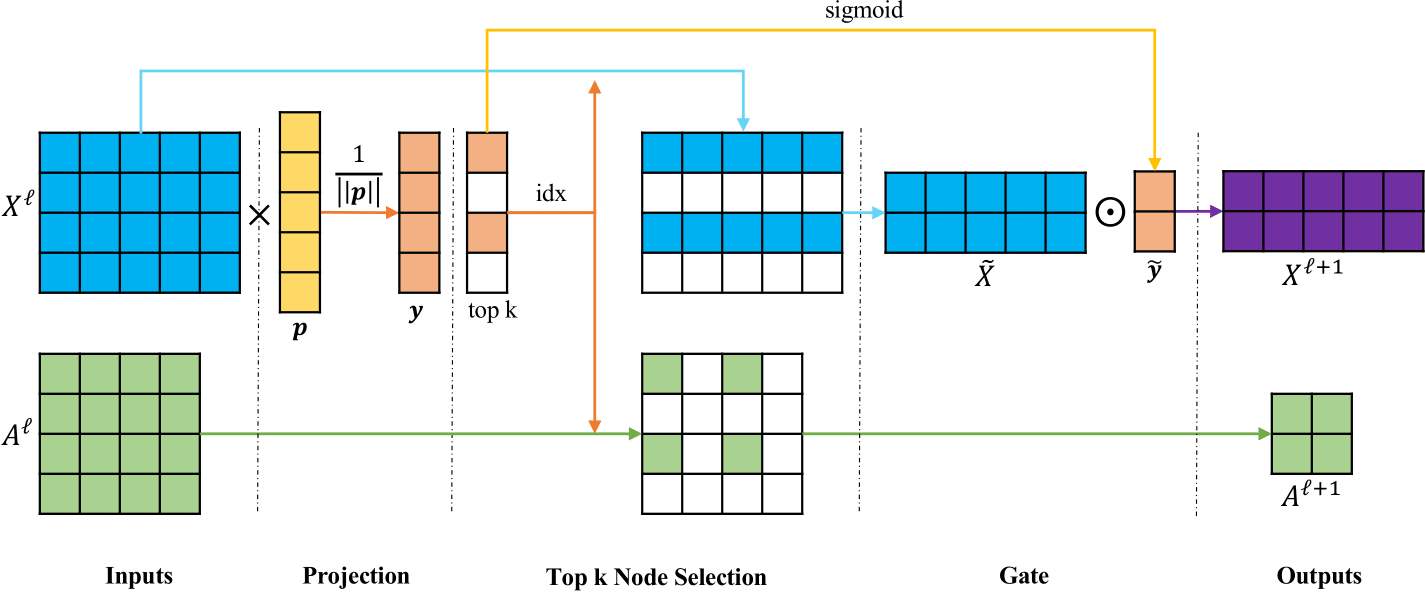
\includegraphics[scale=0.18]{GPool.png}
        \end{column}
        \end{columns}

    \end{frame}

    \begin{frame}
        \frametitle{gUnpool operation}

        \centering
        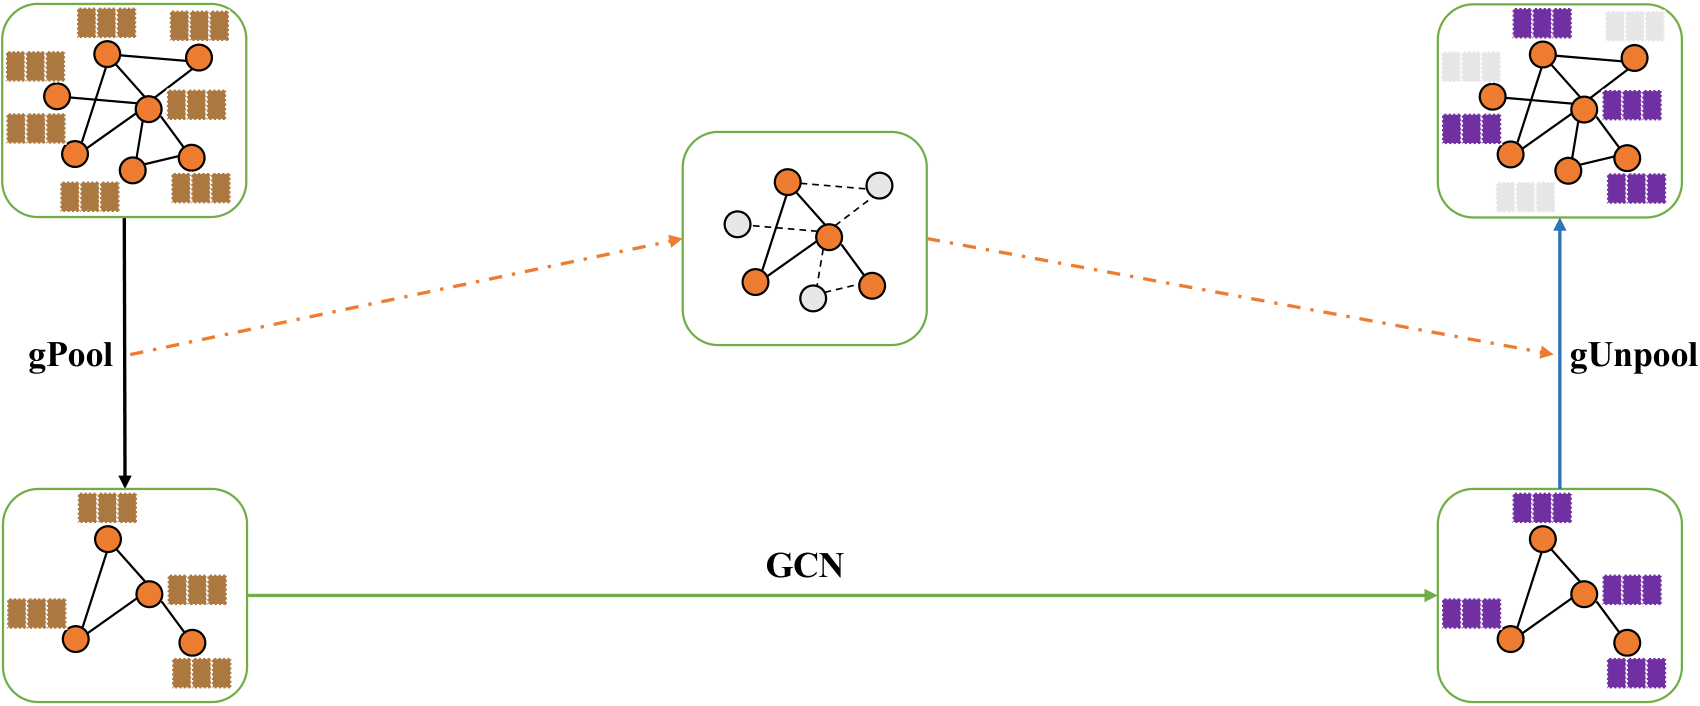
\includegraphics[scale=0.23]{GUnpool.png}

    \end{frame}

    \begin{frame}
        \frametitle{Graph U-Net}

        \centering
        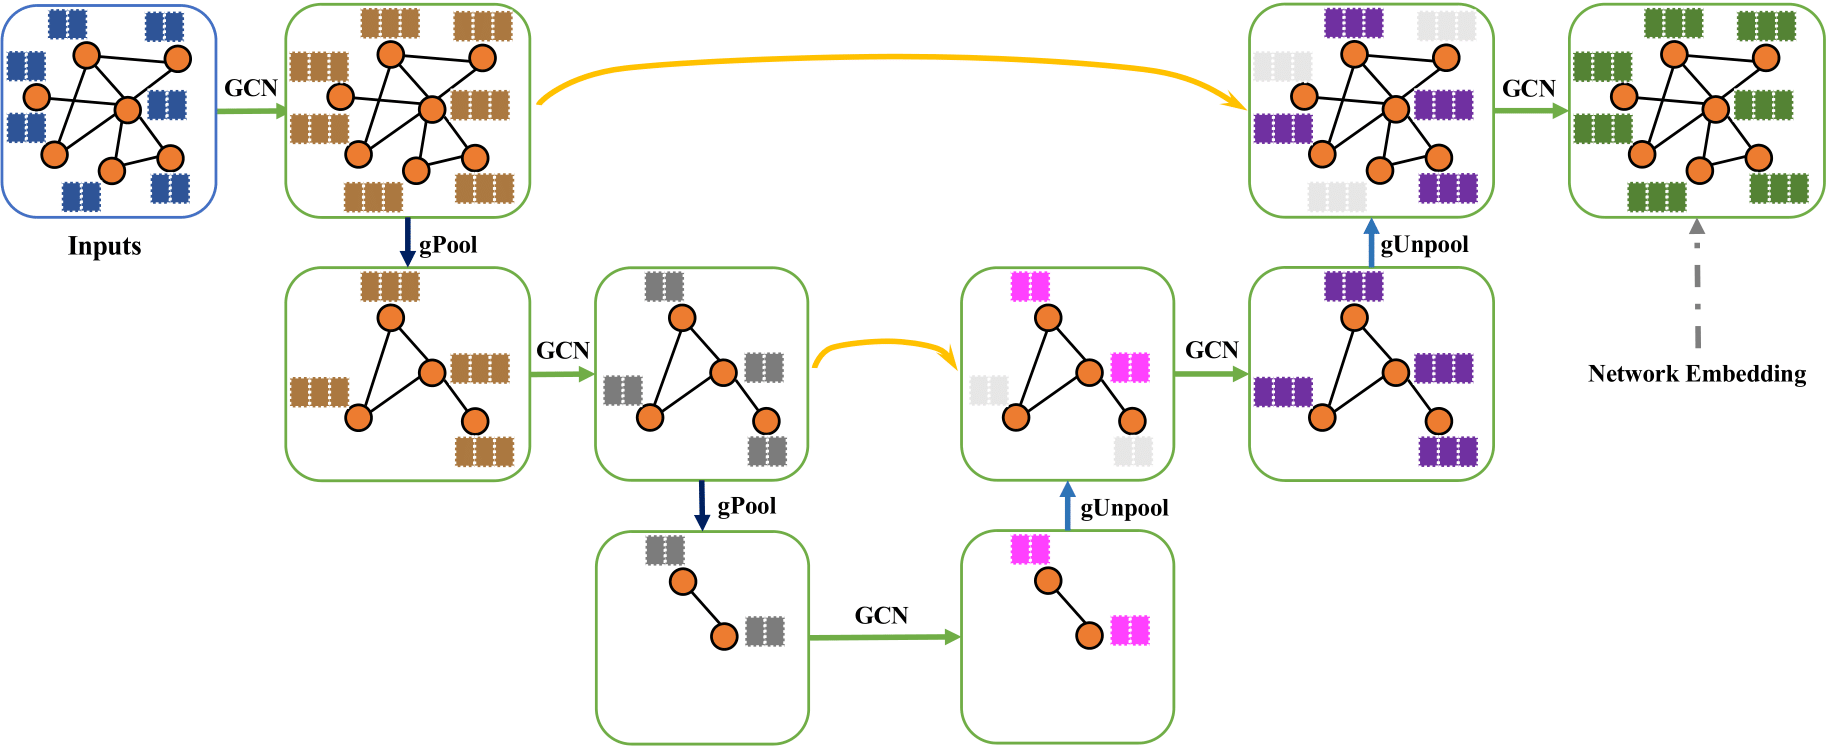
\includegraphics[scale=0.215]{GUnet.png}
    \end{frame}

    \begin{frame}
        \frametitle{Graph Augmentation}

        After the removal of some nodes, the graph may be broken into disconnected parts. To handle this, Graph U-Net
        augments the graph with:

        $$ A^2 = A^lA^l, \quad A^{l+1} = A^2(idx, idx) $$

        Also they empirically found that adding higher weights to self-loops can increase the performance:

        $$ \hat{A} = A + 2I $$
    \end{frame}

    \section{Evaluation}

    \begin{frame}
        \frametitle{Datasets}

        \centering
        \includegraphics[page=6,trim=1cm 18.5cm 1cm 2.5cm,clip,scale=0.7]{Graph U-Net.pdf}
    \end{frame}

    \begin{frame}
        \frametitle{Transductive task (node classification)}

        \centering
        \includegraphics[page=7,trim=1cm 21.2cm 1cm 2.5cm,clip,scale=0.7]{Graph U-Net.pdf}
    \end{frame}

    \begin{frame}
        \frametitle{Inductive task (graph classification)}

        \centering
        \includegraphics[page=7,trim=1cm 16cm 1cm 7.2cm,clip,scale=0.7]{Graph U-Net.pdf}
    \end{frame}

    \begin{frame}
        \frametitle{Ablation study}

        \centering
        \includegraphics[page=8,trim=1cm 20cm 1cm 2.5cm,clip,scale=0.7]{Graph U-Net.pdf}
    \end{frame}

    \begin{frame}
        \frametitle{Parameter size}

        \begin{center}
            \includegraphics[page=8,trim=1cm 13cm 1cm 12cm,clip,scale=0.7]{Graph U-Net.pdf}
        \end{center}

        This suggests that the improvement is not a result of more parameters, and adding gPool and gUnpool will not
        increase the risk of over-fitting.
    \end{frame}

    \appendix

    \begin{frame}
        \frametitle{What I learnt}

        \begin{itemize}
            \setlength{\itemsep}{.8em}
            \item We can find inspirations from CNN techniques when dealing with GNN.
            \item The adjacency matrix can be augmented to impose different weights for links.
        \end{itemize}
    \end{frame}

    \begin{frame}
        \vskip 1.5em

        \centering \huge
        Thank you!
    \end{frame}
\end{document}
